\chapter*{Revision history}

\begin{center}
\begin{tabular}[H]{|l|p{35em}|}
\hline
Version \#  & Description of change (why, what where - a few sentences)\\
\hline
      0.1   & First version is made available via Fronter\\
\hline
\end{tabular}
\end{center}
\newpage

\begin{abstract}
Have you ever realize how secure and safe environment they claim in security product companies' advertisement? Does Anti-Malware software really provide 100 percent security against Malware? As Everybody knows, It is not. Today, it is nothing more than cat and dog fight. Malware authors purpose an new architecture, an new approach and Anti Virus companies just try to fix vulnerabilities. Due to this fact, Parallel and concurrent architectures are elusive field for malware. They are new, trendy, popular, complex. 

In this thesis, we will try to show vulnerabilities on concurrent and parallel cpu schedulers and non-uniform memory architecture. The weaknesses on hardware layer of the computer are hard to be observed by software solution. Therefore; It is time to pay attention for them, since it is not hard to predict that attackers will focus them.

This thesis purpose an offensive security approach, how malware can be evade autonomous malware detection systems, and also purpose and experimental method to detect and mitigate them.
\end{abstract}
\tableofcontents

\chapter{Introduction (1-2 pages)}
The purpose of introduction chapter is giving the readers blueprint of the subject, the problems that we face, the change in the solutions, as well as motivation of its importance. In addition, It also purpose to form proper research question which will guide thesis. 

\subsection{Topic covered by the project}
The thesis purposes an architecture of the malware which process parallel, access memory concurrently, conceal itself systematically, shortly that it is likely to be rocket science. However, everything actually started with a simple mathematical theory by John Von Neumann \cite{von1966theory} and the first example of practical malware is writen by Bob Thomas at BBN, and it was called Creeper 

The malware is abbreviation of malicious software. It could be any piece of code which is defined malicious. There is no formal definition of malicious, it could be some software advertise without any contest or it could be self-producing code piece which aim to distribute itself and steal your private information, and it turned an arm race between power holders today.

With development of the first malware, their counter software are created and anti malware software have evolved with them so far. In this race, malware authors are always one step further, because of security's nature. This race between black and white side raised the bar above. The motivation of the information amount and severity influence both today, and that information can be sometimes vital. 


\subsection{Keywords}
Security, Concurrent Malware Design, Malware, Concurrent, Parallelism and Concurrency

\subsection{Problem description}
The one of the main and indecipherable problem in security discipline is formulating general threat definition and recognizing malicious activity and all this problems unsurprisingly reflect on information and computer security concept. Security is defined by system’s identification, which involve with purpose, crowd, design structures, network model and so on, and today’s information system which is designed with various architectural forms is protected against malware by general purpose protection tools. In the market, The anti malware tools producers focused on pragmatic solutions to survive, but it leads to that most of these tools are utterly reverse engineering process which works on result instead of reason.

With usual and pragmatic signature based methods, there are two mainstream techniques to detect malicious code which are called static and dynamic analysis.Static analysis identifies malwares mainly with code flow graph and data flow graph on stored file which is not processing. However, On the dynamic side it is a bit more tricky to analyze process, because you are working on the running pieces of codes without knowledge of structures and worse than this, it must concern race condition and memory coherency flaws.

The detection methods and techniques have been adequately worked so far because of the simplicity of architectures and usage of the massive generic computers, However, with increasing of the not standardized, parallel and popular devices like arm’s SoC, it is not hard to estimate their new challenges. It is really likely to evade and obfuscate properly your on-the-fly processes with using uncertain charactership of parallel processing, complexity of concurrent programming, and structure of “Non Uniform Memory Architecture”.


\subsection{Justification, motivation and benefits}
If malware designing is superficially considered, you could fall in usual fallacy that It is not beneficial and exactly opposite. However, if we can design it, there is always more skillful author who already abuse this vulnerabilities on the black side of the moon. The work we are obligated to actually proof this vulnerabilities and design counter measure against them. In this way, our blessed motivation is finding possible vulnerabilities, and mitigate or eliminate their risk. Otherwise; if we confront with unknown attack, it could be too late to fix and analyze it. For example, some of the most sensational and beneficial papers are criticize malware as same as the thesis (\cite{moser2007limits},\cite{cavallaro2008limits},\cite{egele2012survey}), and their values are undoubted today. 

\subsection{Research questions}\label{research:questions}

\begin{enumerate}
\item Can a malware model be designed with using parallel and concurrent architecture in order to conceal its presence from detection mechanism?
\item If we can design the mentioned malware, can we build a detection mechanism against these kind of malware's presence?
\item If we build the detection mechanism, What is detection complexity of the algorithms?
\end{enumerate}


\subsection{Planned contributions}
This Master thesis is looking for better understanding on concurrent malware abilities and their counter-measure. Especially, It will try to show how possible to abuse concurrent memory accessing and how durable recent detection kits. It is quite unique work which we have to consider on the future. Ultimate goal is to eliminate any uncertainties which detection methods encounter with concurrent memory accessing.

\section{Related work (3-10 pages)}
This chapter will give an overview of researches about Malware`s self-defense technique, the methods to analyze them, and their application on concurrent architecture. 

\subsection{Malware Self-Defense}
This section will try to give the literature about malware evasion techniques. This techniques are generally antonym solution which are found by malware authors, however, there are enough surveys about known technique. We classified all these methods in six categories which are code obfuscation, code reuse, anti debugging, anti emulator and visualization and covert channel over network traffic. This taxonomy is well defined by Jonathan A.P Marpaung, et al \cite{marpaung2012survey}, yet malware authors used them to protect their own properties. 


Code obfuscation was originally  found for protecting intellectual property\cite{balakrishnan2005code}, but It aims to puzzle code`s binary against merely static analysis and disassembling\cite{nachenberg1996understanding}. The first known obfuscation method used encryption in order to hide its content. It was called Cascade which is seen first 1986\cite{you2010malware}. This simple architecture of the obfuscation is called packing\cite{internotsecurityteam}. It involve with two part of binary which are slub part, in order to decipher and encipher.\cite{marpaung2012survey}. Cascade was using simple XOR encryption and that was increasing performance.

Early of the 1990s , oligomorphism and polimorphism started to show up\cite{you2010malware}. The main idea behind them is basicly transforming their slub part in each attempt of encryption process\cite{nachenberg1996understanding}. Today, there are two type of  polymorphic approach to generate different variants of slub.\cite{li2011mechanisms}
\begin{itemize}
  \item Rewriting the code each time from pseudo-code so it differs code synthetically which is actually transformation based obfuscation.
  \item Self-cipher itself different, order of these ciphers and using different keys.
\end{itemize}
One of the other important milestone of polymorphic malware is Mutation Engine(MtE) is writen by a Bulgarian virus Author, called The Dark Avanger. It was automated obfuscation tool which actually considered impossible in those times.\cite{anonymous1}

There are also several methods to prevent unpacking process. These methods are collected carefully by Peter Ferrie \cite{ferrie2008anti}. These methods are especially obstacle for automated analysis.

Compare with polymorphic methods, metamorphic approach is more complicated. It is transformation based method instead of encryption  approach.\cite{konstantinou2008metamorphic} Fundamentally, it produce different codes which doing same blue printed semantic. That just mitigate detection possibility because of lack of static code. 

Network traffic, which malware produce are generally Achilles heel for malware, because they are generally adequately unique traffics to be identified\cite{marpaung2012survey}. They usually cover their overt malicious traffic with covert channel methods.\cite{rutkowska2006rootkits}

Code reuse attacks are strong attacks because they do not inject any code in them as obfuscation methods did. They aim to use legitimate software to evade themselves. There are there well known applied version which are return-into-libc, return oriented programming and Frankenstein.

Return into libc attacks were demonstrated by solar designer in 1997 as a method of bypassing non executable stack to executable libc libraries\cite{designer1997getting}. It's object is to change the "ret" infrastructure argument to the known address possibly libc library(stdio, system, etc). However, this attack is limited with libc libraries, which we improved with return oriented programming. 

Return oriented programming is more flex version of retur-into-libc attack, which is introduced by Shacham in 2007\cite{shacham2007geometry}. Return oriented programming purpose a programming language with small gadgets(instruction bound) which involve all ability of Turing's machine\cite{roemer2012return}. Frankenstein is one of the novel application of return oriented programming by Vishwath Mohan and Kevin W. Hamlen\cite{mohan2012frankenstein}.

Anti debugging and anti emulator methods are really usual for today's malware. The survey of Chen Xu et al. showed us in 2008, majority of 6900 on-the-air malware could evade their self with exhibiting benign behavior in sandboxes, debuggers, and virtual machines.\cite{chen2008towards}. VM and debuggers are most important element of dynamic analysis techniques in autonomous sector, because it must run the file just before it touch the working environment. Yet, it is not that knotty to determine whether working environment is virtual or not. Fuzzing cpu bechmarks and comparing results entropy is a good way to determine virtual machines.\cite{franklin2008remote}

Rootkits are the piece of malicious code which aims to crack integrity of the system state. The idea of the remaining invisible to the system state is traced backed one of the oldest virus "Brain"\cite{martin2008}. It was changing the boot process and activate virus during booting. "Tequila" and "1689" viruses followed "Brain" in 1991 and 1993\cite{Ducklin1991}. There are NTRootkit and HackerDeffender rootkits today. The proper classification of the rootkit are prepared by Adnan Abdakka\cite{Adnan2011}.



\subsection{Malware analysis methods}

\begin{figure}[h]
    \centering
    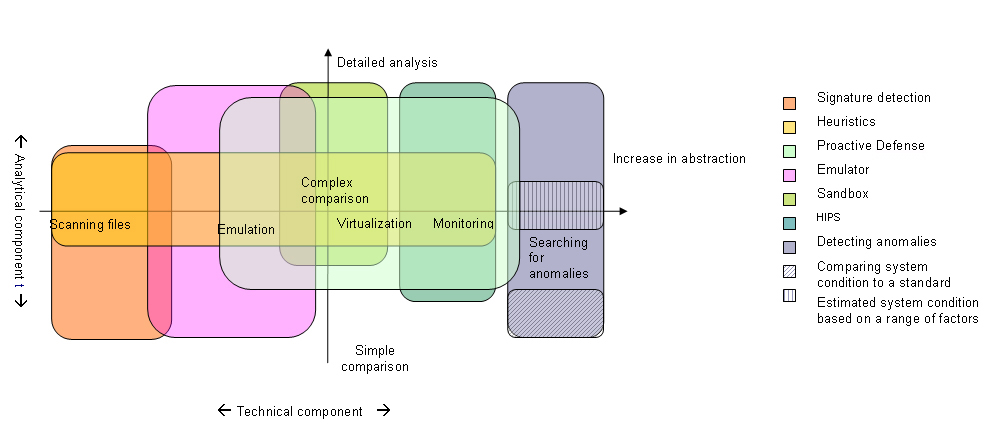
\includegraphics[width=1\textwidth]{alisa_1007_pic1_en.jpg}
    \caption{Detection models \cite{Shevchenko2007detc}}
    \label{fig:awesome_image}
\end{figure}
Malware analysis medhods could be considered two dimensional plane which are "anomaly, signature based detection technique" and "Statistic and dynamic analysis method". 



There are also several applied techniques, which combine terminology above. 
\begin{description}
\item[N-gram] It is a anomaly  based heuristic detection method algorithm. It is a bit costly process and not practical for client side analysis. It could be fit for honey pot analysis \cite{reddy2006n} \cite{abou2004n} \cite{abou2004detection}. They are capable against to zero time malwares and that could makes it futures malware detection system. 
\item[Sequential approach on system and funtion call] This approach is anomaly based dynamic analysis and observing and recording the flow graph of systems and function calls and  try to analysis anomaly behaviors.\cite{kendall2007practical}
\item[Taint] It is also called data flow analysis or data flow graph. It is basic tracking marked data values during execution.\cite{saxena2008efficient}\cite{saxena2008efficient}\cite{smith2007principles}
\item[Control Flow Graph] They are one of the most important arm of commercial autonomous malware detection tools\cite{lee2010detecting} \cite{christodorescu2006static} \cite{christodorescu2005semantics}. After the invention of the polymorphic and metamorphic, syntactic analysis could not bear with them. Then we moved to upper layer of information, semantic layer. Semantic can be representation of code flow, and the routes of the code are adequate to produce signature to identify malware. This methods are a member of static analysis and disassembling and source code analysis job.
\item[Network Monitoring] Malware intention of the communication over network actually big clue to detect them. They generally use unique hostname, ip adress or specific protocol with particular way \cite{marpaung2012survey}.
\end{description}

\section{Choice of methods (2-5 pages)}
This thesis will use a technical approach to the problem. It will use quantitative and model building approach. The methodology consist 8 circular step which are, asking question, building new hypothesis, planning methods, developing software, preparing genering testbed, testing, analyzing, reporting results. In addition to this, the large portion of the time will be given researching related topics, based architecture, and learning tools and technologies. Consequently, the accuracy of the thesis is lies on the proper scientific methodology.

\todo[inline]{ circular diagram will be Drawn here}


To address the first question, designing proper malware evasion technique with concurrent and parallel architecture haven`t been researched well so for, therefore; it will lies on so much experiment and we might have to reflection of other evasion and obfuscation attacks analogy.  We will chose several known malware, which is on air, to  evade them during testing part. We will strong probably use kernel modules and android operating systems for testing bed, however we could linux OS without android layer to simplify and closure test period. In testing step, we will use several anti-virus system such as Avast, Comodo, Norton and compare the result before evasion and after evasion. Testing period might me include mathematical proof depending on evasion or obfuscation method.\todo{Consider involvement of this line during project.} At the end of the each hypothesis` result, which is mean the method for concealing malware, will be reported properly. Each method will be another hypothesis, so we could be proof whether multiple or none successful hypotheses, yet the failed hypothesis could be crucial. There could be also many result which are too barque to proof them or explain their result, these cases could be observed on further work. For semantic knowledge, we could try to show relationship between evasion methods and hybrid approaches.

If we can find successful hypothesis for first question, we observe them in second question. Second question is depend on the first question`s answer. Second questions methodology is actually exactly same circular. It start with defense hypothesis against evasion method. Dynamic and static detection methods must be both considered. The development of the counter algorithms could be proved mathematically, but it can be quite barque to formulate it. In order to prove it, we could design evasion and detection methods` Turing model, however; the main approach of our testing is involved with experimental solution. we will develop planned algorithms prototype. Proper test bed could be provided with lots of malware species.\todo{depending on the found evasion technique, methodology could be shaped again}. We will test our algorithms` prototype with concealed or obfuscated viruses. If it is really necessary, we could prepare also control groups to prove trustworthiness of method, then we have to record result without any intervention. For semantic knowledge, we could try to show relationship between detection methods and hybrid approaches.
\newpage

The last question is a matter of measuring and analyzing algorithms complexity. It is totally mathematical scientific methodology. We have to analyze worst, best and average complexity rate. There are also several Quantitative approaches like measuring resource usage. It could be efficient some system like network which there are lots of uncertainties in.

\section{Milestones, deliverables and resources (2-5 pages)}
This chapter will describe that we plan to demand or supply during the project, such as, what we plan to delivery, how much time should we need.

\subsection{Resources}
This project is involved with only one master research student, one internal supervisor and one external supervisor. Internal supervisor is Prof. Stephan Wolthusen who is excessively capable of malware technologies and their theory. External supervisor is Emre Tinaztepe who is head of  research development department in Comodo AntiVirus. They will support intellectual property of this thesis.

The hardware which we need during this project is quite various. First we need a development board with Samsung Exynos 5420 or 5410 chip which involve with Arm A15 little.Big technology. Arm`s little.Big is an heterogeneous approach for mobile technologies in order to decrease power consumption. There are two brand who produce this boards, Arndale and Odroid. We could also use another parallel architecture called FPGA. The cheapest and optimum FPGA board is Adaptive Parallela. This board has 16 FPGA processor with 1 Arm A7 CPU. We also need one host development computer, Google`s android emulator, IDA Pro software. In addition, We could use Coursera, online education service. In Coursera, Computer Architecture by Princeton University, Hardware software Interaction by Washington University, Heterogeneous Parallel programming by Illinois University.
\subsection{Milestones}
\subsubsection{Pre Education and Utilization}
Pre-education part is the part which utilize us for the future of the project. some of the education topics consist of Kernel Development, Linux-kernel module development, Memory Hierarchy and related attacks, concurrent and parallel programming, return oriented programming, Process scheduling in parallel architectures. Listed Coursera courses is adequate to give relevant background

The estimated time we need is 160 working hour, 4 supervising hour.
\subsubsection{Attack Vector Planning}
Attack planning part is the part which supervisors will be involve critically in. Attack planning is most critical and risk part, we will try to find novel approach to evade malware from anti malware`s scan. 

The estimated time we need is 80 working hour, 4 supervising hour
\subsubsection{Designing  Software Depend on Attack Vector and Testing their result}
We will produce applied version of our theoretical attack vectors with the propose of test and analysis the success of hypothesis. It will require C, Assembly and Linux-Android intervals knowledge.

The estimated time we need is 80 working hour, 2 supervising hour 
\subsubsection{Designing  Defense Against Successful Attack and Testing their result}
In this part, we will try to find answer for second question of the research. Depending on attack vector, it could require various skills. Probably, it will require Python, linux kernel knowledge.

The estimated time we need is 80 working hour, 4 supervising hour 
\subsubsection{Complexity analysis and proofs}
The complexity Analysis and proofs will be calculated in this part. Some part of this analysis could be left to further work. 

The estimated time we need is 80 working hour, 2 supervising hour 

\subsubsection{Reporting}
All knowledge related with thesis must be projected semantically in thesis report. The report will include what we found, what we mange to do, what we can not, also it must present related knowledge, figures, diagrams and charts. In order to use image files in the thesis we must request access and use right. Organization could be really puzzled work if you do not give enough care on. We should prepare first draft before final version and distribute reviewer.  

The estimated time we need is 80 working hour, 2 supervising hour 

\subsection{Deliverables}
The main deliverable of the project is master thesis. There are two reviewer of this thesis Prof. Stephan Wolthusen and My fellow student, Oyvind Nordhaug. The reviewer are capable of relevant background and fortunately they will positively criticize thesis . We could classify the thesis in three part. Introduction, background, payload.

Introduction part's first draft is actually written, when we wrote current sections. It include Abstraction, Introduction of the project, Problem Description, Research questions, and Related works. 

Background part is include Concurrent, parallel architectures and programming such as Heterogeneous and FPGA, Non uniform memory architectures and their attacks, Malware analysis techniques and related evasion techniques.

Payload is the part actually emphasis our work. It will consist attack vectors, their theory, applied source code, defense theory, metrics, and etc.


\section{Feasibility study (1/2-3 pages)}

This thesis will try to cover the gap in concurrent malware analysis. It was actually one of the unique research on this area, however; there is a master thesis belong last year which is supervised by Prof. Mr. Stephen Wolthusen\cite{Tsopokis2012Concurrent}. It gives us corpus collection about concurrent memory inspection and showed there could be vulnerabilities. 

Vulnerability analysis is always risky work, but in the worst case, whole experiment is going to give particular knowledge whether succeed or not. 

Also as we know from our computation experiment, concurrent and parallel architecture are the most baroque part which mean complicated but efficient. This complexity is always enemy of security and we do not suppose we are doing an Inexpedient job.
\section{Risk analysis (1/2-2 pages)}
In this project, there five inevitable risks which we can face during development.

\begin{itemize}
\item The thesis is highly dependent on the hardware, and the cost of the hardware constitute risk on its own. Any case of hardware defect leads to comprise obstacle.
\item Hardware dependency is also leads to logistical and time consuming risk which could result with latency on submit time.
\item Firmware codes which we are planning to work on are mostly undocumented. We could discover their usage by proper reverse engineering and fuzzing process when required, however it is obviously manpower.
\item Most important and highlighting risk is there isn't proper research on this particular area. That means there are strongly possibly hidden risks which could cause other mental and physical result.
\item During testing and purification part, Anti-malware tools could come out with unreliable result. To analyze result properly, we may need to inspect mentioned tools with reverse engineering process which could violate proper usage agreement. To mitigate that kind of risks, we could request research agreement from companies.  
\end{itemize}

\section{Ethical and legal considerations (1/4-1 page)}
The content of this document could be used in order to malicious purpose, but any matter or information could be misused in the life and ignorance is not known well as a defense strategy. In this purpose, this thesis aims to enlighten security specialist and system developers against recent way of the possible attacks. 

However, in order to act ethical responsibility, we tried to eliminate practice of tools and piece of codes which could leads malicious usage. In any case, there is no doubt that it is critical to discover and publish vulnerabilities which could cause deep impact before malicious people discover and abuse them.

\begin{quote}

"Virus don't harm, ignorance does."\\
- VxHeaven
\end{quote}
